\documentclass[border=6pt]{standalone}
% ---------------------------------------------------------------------------
% tikzpreamble.tex -- shared by main.tex and by every standalone in tikz/
% ---------------------------------------------------------------------------
\usepackage{amsmath}
\usepackage{amssymb}
\usepackage{tikz}
\usepackage{circuitikz}
\usetikzlibrary{arrows.meta,calc,positioning,decorations.pathmorphing,decorations.pathreplacing,
                decorations.markings,patterns,angles,quotes,fit,
                shapes.geometric,shapes.misc,backgrounds,intersections}

\ctikzset{bipoles/length=0.85cm}
\ctikzset{resistors/scale=0.85}
\ctikzset{capacitors/scale=0.9}

\tikzset{
  wire/.style      = {line width=0.7pt},
  dashedwire/.style= {line width=0.7pt, densely dashed},
  term/.style      = {circle, draw, line width=0.6pt, fill=white,
                      inner sep=0pt, minimum size=4.5pt},
  node dot/.style  = {circle, fill=black, inner sep=0pt, minimum size=4pt},
  boxlabel/.style  = {font=\sffamily\small},
  annot/.style     = {font=\small, align=left},
  phasor/.style    = {-{Stealth[length=3.2mm,width=2.2mm]}, line width=1.1pt},
  thinphasor/.style= {-{Stealth[length=2.6mm,width=1.8mm]}, line width=0.7pt},
  axis line/.style = {-{Stealth[length=2.6mm,width=1.8mm]}, line width=0.6pt},
  guide/.style     = {densely dashed, line width=0.4pt, gray},
}
\usepackage{siunitx}

\definecolor{condband}{RGB}{150,155,235}
\definecolor{valband}{RGB}{232,72,72}
\definecolor{overlapband}{RGB}{112,55,150}
\begin{document}
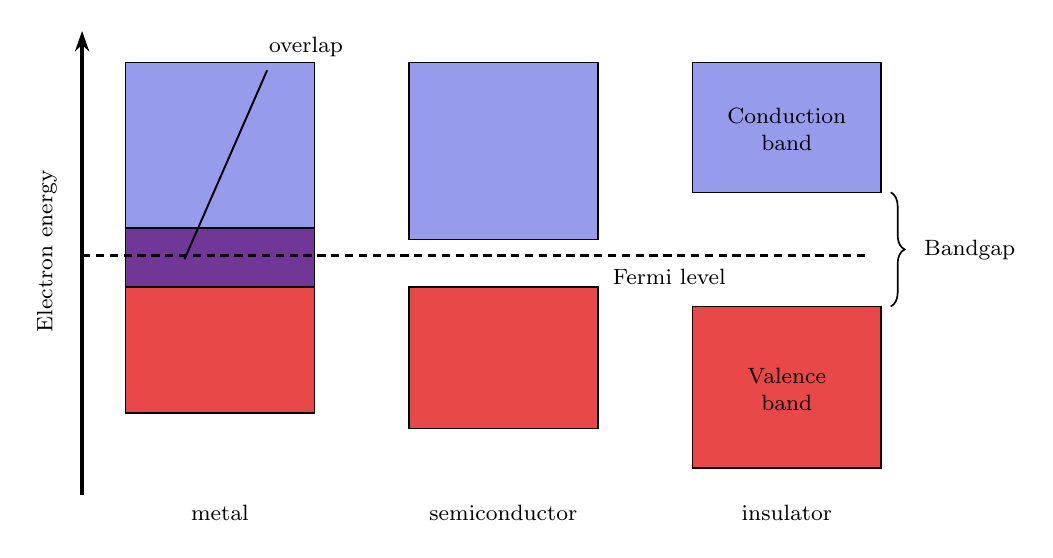
\begin{tikzpicture}[every node/.style={font=\small}]
  \def\bw{2.4}   % band width

  \draw[axis line,line width=1.2pt] (-0.55,-0.5) -- (-0.55,5.4);
  \node[rotate=90,anchor=south,font=\footnotesize] at (-0.75,2.6) {Electron energy};

  % ---------------- metal -------------------------------------------------
  \begin{scope}[shift={(0,0)}]
    \filldraw[fill=condband,draw=black,line width=0.6pt] (0,2.55) rectangle (\bw,5.0);
    \filldraw[fill=overlapband,draw=black,line width=0.6pt] (0,2.15) rectangle (\bw,2.9);
    \filldraw[fill=valband,draw=black,line width=0.6pt] (0,0.55) rectangle (\bw,2.15);
    \node[anchor=north,font=\footnotesize] at (\bw/2,-0.5) {metal};
    \draw[line width=0.7pt] (0.75,2.5) -- (1.8,4.9);
    \node[anchor=south west,font=\footnotesize] at (1.7,4.95) {overlap};
  \end{scope}

  % ---------------- semiconductor ----------------------------------------
  \begin{scope}[shift={(3.6,0)}]
    \filldraw[fill=condband,draw=black,line width=0.6pt] (0,2.75) rectangle (\bw,5.0);
    \filldraw[fill=valband,draw=black,line width=0.6pt] (0,0.35) rectangle (\bw,2.15);
    \node[anchor=north,font=\footnotesize] at (\bw/2,-0.5) {semiconductor};
  \end{scope}

  % ---------------- insulator --------------------------------------------
  \begin{scope}[shift={(7.2,0)}]
    \filldraw[fill=condband,draw=black,line width=0.6pt] (0,3.35) rectangle (\bw,5.0);
    \node[align=center,font=\footnotesize] at (\bw/2,4.15) {Conduction\\ band};
    \filldraw[fill=valband,draw=black,line width=0.6pt] (0,-0.15) rectangle (\bw,1.9);
    \node[align=center,font=\footnotesize] at (\bw/2,0.85) {Valence\\ band};
    \node[anchor=north,font=\footnotesize] at (\bw/2,-0.5) {insulator};
    \draw[decorate,decoration={brace,amplitude=5pt},line width=0.6pt]
         (\bw+0.12,3.35) -- (\bw+0.12,1.9);
    \node[anchor=west,font=\footnotesize] at (\bw+0.42,2.62) {Bandgap};
  \end{scope}

  % ---------------- Fermi level ------------------------------------------
  \draw[densely dashed,line width=1.1pt] (-0.55,2.55) -- (9.4,2.55);
  \node[anchor=north west,font=\footnotesize,fill=white,inner sep=1pt] at (6.15,2.42) {Fermi level};
\end{tikzpicture}
\end{document}
